\documentclass[12pt,a4paper]{report}
\usepackage[utf8]{inputenc}
\usepackage[T1]{fontenc}
\usepackage{graphicx}
\graphicspath{{figures/}}
\usepackage{booktabs}
\usepackage{amsmath}
\usepackage{hyperref}
\usepackage{caption}
\usepackage{subcaption}
\usepackage[margin=2.5cm]{geometry}
\usepackage{setspace}
\onehalfspacing
\usepackage[style=ieee,backend=biber]{biblatex}
% \addbibresource{references.bib}

\title{Multi-Modal Drone Detection with Trust-Aware Sensor Fusion and Confuser-Aware Gating}
\author{Ahmed Eltayeb}
\date{2026}

\begin{document}
\maketitle
\tableofcontents
\listoffigures
\listoftables

% ======================================================================
% CHAPTER 1 — INTRODUCTION
% ======================================================================
\chapter{Introduction}
\label{ch:introduction}

\section{Background}

The rapid proliferation of commercial unmanned aerial vehicles (UAVs) has created an urgent need for automated aerial surveillance systems capable of detecting drones in real time. Consumer drones are readily available, inexpensive, and increasingly used for purposes ranging from recreational photography to agricultural monitoring. However, their accessibility also introduces security risks: drones have been used for unauthorized surveillance, smuggling across borders, disrupting airport operations, and posing collision hazards to manned aircraft~\cite{TODO_counterUAS_survey}. Regulatory frameworks continue to evolve, but enforcement relies heavily on the ability to \emph{detect} rogue drones before they cause harm.

Visual detection using camera-based systems offers several advantages over radar and radio-frequency (RF) approaches: cameras are passive, inexpensive, and can provide rich contextual information about the detected object. Modern deep learning detectors---particularly the YOLO family of single-stage architectures---have demonstrated strong performance on drone detection benchmarks. However, single-modality visual detection faces a fundamental challenge: \emph{confuser objects}. Birds, airplanes, helicopters, and other airborne objects share visual characteristics with drones at typical detection distances. A detector optimized for high recall on drones inevitably generates false positives on these confuser categories.

This thesis addresses the confuser problem through a multi-modal, multi-stage detection architecture that combines RGB and thermal infrared (IR) imagery with learned trust-aware fusion. Rather than attempting to build a single detector that perfectly discriminates drones from confusers, the system employs a cascade of specialized components: high-recall base detectors, a trust classifier that determines which modality to believe, and a confuser-specific patch verifier that provides the final discrimination layer.

\section{Problem Statement}

Single-modality drone detectors hallucinate extensively on confuser objects. On the Svanstr\"om evaluation dataset at inference resolution 1280, the baseline RGB detector fires on 94.4\% of bird frames, 74.6\% of airplane frames, and 66.2\% of helicopter frames (Table~\ref{tab:rgb_comparison}). Retraining the detector with hard-negative mining only partially mitigates this: bird hallucination remains at 94.2\% even after aggressive confuser augmentation, while drone recall drops from 0.959 to 0.950. A more aggressive retraining strategy (retrained\_v2) collapses drone recall to 0.306---a 68\% reduction---rendering the detector unusable.

This presents a fundamental dilemma: high-recall detectors hallucinate, and high-precision retraining destroys recall. The research question motivating this work is:

\begin{quote}
\emph{Can a multi-stage fusion architecture suppress confuser false positives while preserving high drone recall, without requiring the base detector to learn the discrimination task?}
\end{quote}

\section{Research Objectives}
\begin{enumerate}
    \item Design and implement a multi-modal (RGB + thermal IR) drone detection pipeline
          with trust-aware sensor fusion.
    \item Develop confuser-specific discrimination layers (trust classifier + patch verifier)
          to suppress false positives from birds, airplanes, and helicopters.
    \item Evaluate the system through rigorous, reproducible ablation studies with
          per-component provenance tracking.
    \item Build a human-in-the-loop label review tool to ensure training data quality
          and demonstrate iterative model-data co-evolution.
    \item Demonstrate production readiness through a real-time PySide6 GUI capable of
          processing paired RGB+IR video streams.
\end{enumerate}

\section{Contributions}
\begin{itemize}
    \item A trust-aware fusion classifier that dynamically selects which sensor modality
          to trust per frame, reducing confuser fire rates from 52.1\% (raw YOLO) to 1.6\%
          (post-classifier) on out-of-distribution confuser images---a 97\% suppression rate
          at the classifier stage alone.
    \item A 4-class patch verifier for bird/airplane/helicopter/other discrimination
          at the alert gate, providing a further 50\% reduction in residual false positives
          (1.6\% $\rightarrow$ 0.8\%).
    \item A scoring-rule audit revealing a 28-percentage-point F1 swing between
          evaluation methodologies (dual vs.\ trust\_aware scoring), establishing the importance
          of transparent metric reporting in detection systems.
    \item A human-in-the-loop label reviewer enabling systematic dataset curation,
          demonstrated through five iterations of IR model development that improved
          mAP50 from 0.900 to 0.958.
    \item A data-centric AI workflow where model-assisted labeling, human review of
          false positives, and targeted data acquisition form an iterative loop that
          progressively improves both dataset quality and model performance.
    \item Fully reproducible evaluation infrastructure with per-run JSON manifests
          linking every reported metric to its source data and configuration.
\end{itemize}

\section{Thesis Outline}

Chapter~\ref{ch:literature} reviews the literature on object detection architectures, drone detection methods, multi-modal sensor fusion, and human-in-the-loop machine learning. Chapter~\ref{ch:architecture} presents the system architecture, including the design rationale for the multi-stage cascade and the trust-aware fusion formulation. Chapter~\ref{ch:components} details the design and training of each pipeline component: the RGB and IR detectors, the trust classifier, the confuser patch verifier, and the human-in-the-loop label reviewer. Chapter~\ref{ch:ood} analyses out-of-distribution generalization, including the unexpected finding that the IR model---trained exclusively on thermal data---performs effectively on grayscale-converted RGB images. Chapter~\ref{ch:setup} describes the experimental setup, datasets, evaluation metrics, and the scoring-rule audit. Chapter~\ref{ch:results} presents the main results and ablation studies. Chapter~\ref{ch:discussion} discusses the architectural implications, limitations, and future work. Chapter~\ref{ch:conclusion} concludes.

% ======================================================================
% CHAPTER 2 — LITERATURE REVIEW
% ======================================================================
\chapter{Literature Review}
\label{ch:literature}

\section{Object Detection Architectures}
% YOLO family evolution (v1 through v11/Ultralytics).
% Single-stage vs two-stage detectors. Why YOLO for real-time drone detection.
% CITE: Redmon et al. (2016), Ultralytics YOLOv8/v11 documentation.

\section{Drone Detection in Aerial Surveillance}
% Survey of existing approaches: radar, acoustic, RF, visual.
% RGB-based drone detection challenges: small object size, background clutter,
%   confuser objects (birds, aircraft).
% CITE: Anti-UAV benchmark paper, Svanström et al. dataset paper.

\section{Thermal Infrared Imaging for Detection}
% Advantages of IR: illumination invariant, thermal signature.
% Limitations: lower spatial resolution, atmospheric effects.
% DATA BACKING: IR model achieves 0.961 F1 on Svanström vs RGB 0.949 —
%   but IR also hallucinates (22\% on confuser set).
%   Source: EVIDENCE_LEDGER §4, confuser_test_hallucination.csv

\section{Multi-Modal Sensor Fusion}
% Early vs late vs decision-level fusion.
% Trust-based fusion: dynamically weighting modalities.
% CITE: multi-modal fusion surveys, attention-based fusion methods.

\section{Hard-Negative Mining}
% Training with confuser images to improve specificity.
% Online vs offline mining strategies.
% CITE: Shrivastava et al. (2016) OHEM, focal loss (Lin et al., 2017).
% DATA BACKING: three RGB retrains showed diminishing returns —
%   hardneg_v3more only improved helicopter halluc (66→42\%), not birds (94→94\%).
%   Source: svanstrom_1280_by_category.csv

\section{Confidence Calibration and Scoring Rules}
% Why confidence scores are not probabilities.
% Impact of evaluation methodology on reported metrics.
% CITE: Guo et al. (2017) calibration, IoU vs IoP scoring comparisons.
% DATA BACKING: dual vs trust\_aware scoring = 28pp F1 swing.
%   Source: eval/results/_ablation/.../E_scoring/

\section{Human-in-the-Loop Machine Learning}
% Active learning, label quality, annotation tools.
% Why systematic label review matters for small datasets.
% CITE: Settles (2009) active learning survey, data-centric AI (Andrew Ng).

% ======================================================================
% CHAPTER 3 — SYSTEM ARCHITECTURE
% ======================================================================
\chapter{System Architecture}
\label{ch:architecture}

\section{Architecture Overview}

The detection pipeline processes paired RGB and thermal IR video streams through a multi-stage cascade, where each stage contributes measured, additive confuser suppression. The architecture comprises five principal components:

\begin{enumerate}
    \item \textbf{RGB Detector}: A YOLOv26n model trained on RGB imagery, optimized for maximum drone recall.
    \item \textbf{IR Detector}: A YOLOv26n model finetuned on thermal infrared data, providing illumination-invariant detection.
    \item \textbf{Trust Classifier}: An XGBoost classifier that takes detection signals from both modalities and determines which detections to trust.
    \item \textbf{Patch Verifier}: A 4-class CNN that examines detection crops to discriminate confuser categories (bird, airplane, helicopter) from drones.
    \item \textbf{Temporal Gate}: A sliding-window smoother that suppresses isolated, non-persistent detections.
\end{enumerate}

% PLACEHOLDER FIGURE: Full pipeline block diagram
\begin{figure}[htbp]
    \centering
    % \includegraphics[width=\textwidth]{figures/pipeline_block_diagram.png}
    \fbox{\parbox{0.9\textwidth}{\centering\vspace{3cm}
        \textbf{[PLACEHOLDER: Fig 3.1]} Full pipeline block diagram\\
        RGB YOLO $\rightarrow$ IR YOLO $\rightarrow$ Trust Classifier $\rightarrow$
        Patch Verifier $\rightarrow$ Temporal Gate $\rightarrow$ Alert
    \vspace{3cm}}}
    \caption{Multi-stage drone detection pipeline. Each stage contributes measured,
             additive confuser suppression (Section~\ref{sec:cumulative_results}).}
    \label{fig:pipeline}
\end{figure}

On out-of-distribution confuser images, the pipeline reduces the false positive fire rate from 52.1\% (Stage~1, raw YOLO detections) to 1.6\% (Stage~2, post-classifier) to 0.8\% (Stage~3, post-patch verifier)---a cumulative 98.4\% suppression (Section~\ref{sec:cumulative_results}). Critically, this suppression is achieved \emph{without retraining} the base detectors, preserving their high drone recall (0.959 on Svanstr\"om).

\section{Design Rationale}
\label{sec:design_rationale}

The central architectural decision is to \emph{ship the high-recall detector and let downstream components handle precision}. This ``fail-open'' design is motivated by a key empirical observation: lost recall cannot be recovered by downstream processing, but false positives can always be filtered.

Table~\ref{tab:rgb_comparison} demonstrates this tradeoff concretely. The baseline RGB detector achieves 0.959 drone recall but hallucinates on 94.4\% of bird frames. An aggressively retrained model (retrained\_v2) reduces bird hallucination to 3.4\% but collapses drone recall to 0.306---a 68\% loss. No amount of downstream processing can recover the drones that the detector missed.

By contrast, the multi-stage pipeline takes the high-recall baseline and progressively strips away false positives at each stage:
\begin{itemize}
    \item Stage~1 (YOLO): 52.1\% confuser fire rate, drone recall 0.959
    \item Stage~2 (+ Trust Classifier): 1.6\% confuser fire rate, drone recall maintained
    \item Stage~3 (+ Patch Verifier): 0.8\% confuser fire rate, drone recall 0.816
\end{itemize}

The net result is a 98.4\% reduction in confuser false positives while retaining the majority of drone detections. This validates the design philosophy: precision is the burden of the classifier, not the detector.

\section{Trust-Aware Fusion}
\label{sec:trust_fusion}

Rather than simply averaging or voting between modality detections, the system employs a learned trust classifier that maps frame-level features to a modality trust decision. The classifier outputs one of four classes:

\begin{itemize}
    \item \textbf{reject\_both}: Neither modality's detection is trustworthy (likely a confuser).
    \item \textbf{trust\_rgb}: Only the RGB detection is reliable.
    \item \textbf{trust\_ir}: Only the IR detection is reliable.
    \item \textbf{trust\_both}: Both modalities agree and are trustworthy.
\end{itemize}

% PLACEHOLDER FIGURE: Trust classifier decision flow
\begin{figure}[htbp]
    \centering
    \fbox{\parbox{0.8\textwidth}{\centering\vspace{2.5cm}
        \textbf{[PLACEHOLDER: Fig 3.2]} Trust classifier 4-class decision flow\\
        Input features $\rightarrow$ XGBoost $\rightarrow$
        \{reject\_both, trust\_rgb, trust\_ir, trust\_both\}
    \vspace{2.5cm}}}
    \caption{Trust classifier maps 40 frame-level features to a modality trust decision.
             Top feature: \texttt{ir\_detected} (49\% importance).}
    \label{fig:trust_flow}
\end{figure}

This 4-class formulation is superior to a binary ``drone or not'' classifier because it captures \emph{when} each modality is reliable. For example, in night-time conditions, the classifier learns that RGB detections are unreliable (no visible-light signal) and should be disregarded in favour of IR. Conversely, in certain thermal conditions where IR produces spurious detections, the classifier can fall back to RGB-only trust. The most informative feature is \texttt{ir\_detected} (49\% importance), indicating that IR detection presence is the single strongest signal for trust decisions.

\section{Alert-Gate Cascade}
\label{sec:alert_gate}

The patch verifier operates as an \emph{alert gate}: it is only consulted when the trust classifier has already accepted a detection. This ``alert-gate-only'' design was chosen over a ``filter-then-classify'' approach based on empirical testing. Per-frame patch filtering prior to the trust classifier incurred an approximately 1-percentage-point F1 penalty due to premature rejection of marginal but genuine drone detections. By positioning the patch verifier after the trust classifier, only high-confidence but potentially confuser-like detections are subjected to the additional verification step.

In production, this translates to minimal additional latency: the patch verifier's CNN inference is triggered only on frames where the trust classifier has fired an alert, which represents a small fraction of total frames in typical surveillance scenarios.

\section{Temporal Smoothing}
\label{sec:temporal}

The temporal gate implements a sliding-window smoother with a 5-of-6 alert threshold and configurable cooldown periods. A drone alert is only raised if at least 5 of the last 6 frames contain positive detections from the trust classifier. This suppresses isolated, non-persistent firings that are characteristic of confuser objects passing through the field of view.

Temporal smoothing is not included in the cumulative suppression chart (Figure~\ref{fig:cumulative_confuser}) because the evaluation framework processes frames independently, without temporal ordering. In production deployment with video streams, the temporal gate provides an additional layer of confuser rejection that further reduces the false positive rate. Quantifying this effect requires ordered video evaluation, which is identified as future work.

\section{Resolution Dependency}
\label{sec:resolution}

Inference resolution is a critical but often overlooked hyperparameter for small-object detection. The Svanstr\"om dataset has a native resolution of 640$\times$512, meaning drones occupy very small pixel areas. At the default YOLO inference resolution of 640 pixels, the RGB detector achieves only 0.072 drone recall---effectively blind. Increasing inference resolution to 1280 pixels raises recall to 0.959, a 13.3$\times$ improvement (Figure~\ref{fig:resolution}).

This is not a model defect but a geometric inevitability: when the input image is already 640 pixels wide, downscaling to 640$\times$640 inference resolution provides no effective resolution gain. The drones are too small to activate the detector's feature maps. At 1280$\times$1280, YOLO's internal letterboxing upscales the 640$\times$512 image by approximately 2$\times$, providing sufficient resolution for the detector to identify drone features.

All results in this thesis use \texttt{imgsz=1280} for the RGB detector on Svanstr\"om data unless otherwise noted. The IR detector uses \texttt{imgsz=640} by default, as thermal imagery typically has sufficient contrast for detection at lower resolutions.

% ======================================================================
% CHAPTER 4 — COMPONENT DESIGN AND TRAINING
% ======================================================================
\chapter{Component Design and Training}
\label{ch:components}

\section{RGB Drone Detector}

\subsection{Model Architecture}

The RGB drone detector uses the YOLOv26n architecture from Ultralytics---the nano variant optimized for inference speed while maintaining competitive detection accuracy. The model is configured as a single-class detector (class~0: ``drone'') and was initially pretrained on the COCO dataset before finetuning on a custom drone detection corpus.

\subsection{Training Data}

The RGB detector was trained on a composite dataset (\texttt{drone\_mixed.yaml}) comprising 137,506 training images drawn from multiple sources: the Anti-UAV RGBT dataset (RGB frames), Roboflow community drone datasets, and manually curated aerial footage. Importantly, no Svanstr\"om data was included in the RGB training set, making the Svanstr\"om evaluation a genuine out-of-distribution test for this component.

Training used the AdamW optimizer with an initial learning rate of 0.001, batch size 48, and inference resolution \texttt{imgsz=640}. Mosaic augmentation (probability 0.33) and random erasing (probability 0.4) were enabled to improve robustness.

% PLACEHOLDER FIGURE: RGB training curves
\begin{figure}[htbp]
    \centering
    \fbox{\parbox{0.8\textwidth}{\centering\vspace{2.5cm}
        \textbf{[PLACEHOLDER: Fig 4.1]} RGB baseline training curves\\
        Source: \texttt{RGB model/Yolo26n\_trained/results.csv}
    \vspace{2.5cm}}}
    \caption{Training loss and mAP curves for the baseline RGB drone detector.}
    \label{fig:rgb_training}
\end{figure}

\subsection{Three Training Iterations}

Three variants of the RGB detector were developed, which can be framed as an intentional recall-precision tradeoff ablation:

\begin{enumerate}
    \item \textbf{Baseline}: Trained on the original drone corpus without confuser images. This model achieves the highest drone recall (0.959) but hallucinates extensively on confuser objects.
    \item \textbf{hardneg\_v3more}: Retrained with aggressive hard-negative mining, incorporating confuser images (birds, airplanes, helicopters) as negative examples. This reduced helicopter hallucination from 66.2\% to 41.9\% but left bird hallucination unchanged at 94.2\%.
    \item \textbf{retrained\_v2}: A complete retraining with heavy confuser augmentation, designed to teach the detector to reject confusers. While bird hallucination dropped to 3.4\%, drone recall collapsed to 0.306---a 68\% reduction.
\end{enumerate}

\begin{table}[htbp]
    \centering
    \caption{RGB model variants on Svanstr\"om @ imgsz=1280. Baseline achieves highest
             drone recall; retrained\_v2 collapses to 0.306.
             Source: \texttt{svanstrom\_1280\_by\_category.csv}.}
    \label{tab:rgb_comparison}
    \begin{tabular}{lccccc}
        \toprule
        Model & Drone R & Drone P & Bird Halluc & Airplane Halluc & Heli Halluc \\
        \midrule
        baseline     & \textbf{0.959} & 0.940 & 94.4\% & 74.6\% & 66.2\% \\
        hardneg\_v3  & 0.950          & 0.941 & 94.2\% & 64.7\% & 41.9\% \\
        retrained\_v2 & 0.306         & 0.943 & 3.4\%  & 5.6\%  & 4.5\%  \\
        \bottomrule
    \end{tabular}
\end{table}

The key insight from this ablation is that hard-negative mining has diminishing returns. Birds are geometrically and texturally similar to drones at typical detection distances, and the YOLO feature extractor cannot reliably discriminate them at the single-stage detection level. This motivated the architectural decision to handle confuser discrimination downstream (Section~\ref{sec:design_rationale}): the baseline model was selected for production, and confuser suppression was delegated to the trust classifier and patch verifier.

\section{IR Drone Detector}

\subsection{Model Architecture and Finetuning}

The IR detector uses the same YOLOv26n architecture as the RGB detector, finetuned on thermal infrared imagery. The model was iteratively developed through the human-in-the-loop process described in Section~\ref{sec:hitl}, with the final production model (\texttt{v3b}) achieving 0.946 mAP50 on the IR validation set.

The IR detector operates at \texttt{imgsz=640} by default. Unlike RGB imagery, thermal images have inherently high contrast between the drone (warm body) and the background, meaning lower inference resolution is typically sufficient.

% PLACEHOLDER FIGURE: IR training curves
\begin{figure}[htbp]
    \centering
    \fbox{\parbox{0.8\textwidth}{\centering\vspace{2.5cm}
        \textbf{[PLACEHOLDER: Fig 4.2]} IR model training curves\\
        Source: \texttt{runs/corrective\_finetune/finetune\_v3b/results.csv}
    \vspace{2.5cm}}}
    \caption{Training curves for the IR drone detector (corrective finetune v3b).}
    \label{fig:ir_training}
\end{figure}

\subsection{IR vs RGB: Complementary Strengths}

The RGB and IR modalities have complementary failure modes, which motivates the multi-modal architecture:

\begin{itemize}
    \item \textbf{Illumination}: The RGB detector fails in low-light and night-time conditions, where the image contains insufficient visible-light signal. The IR detector is illumination-invariant, relying on thermal emission rather than reflected light.
    \item \textbf{Confuser discrimination}: On the confuser test set, the IR model hallucinates on only 22.2\% of images versus 53.0\% for the RGB model---a 2.4$\times$ reduction (Table~\ref{tab:ir_grayscale}). This is because confuser objects (birds, airplanes, helicopters) have different thermal signatures from drones, whereas their visual appearance is similar.
    \item \textbf{Spatial resolution}: RGB imagery provides higher spatial resolution and colour information, which aids detection in daylight conditions where thermal contrast may be low.
\end{itemize}

% PLACEHOLDER FIGURE: RGB fails at night, IR succeeds
\begin{figure}[htbp]
    \centering
    \fbox{\parbox{0.9\textwidth}{\centering\vspace{2.5cm}
        \textbf{[PLACEHOLDER: Fig 4.3]} Side-by-side: RGB misses drone at night,
        IR detects it clearly.\\
        Source: Anti-UAV night sequence frames (TBD)
    \vspace{2.5cm}}}
    \caption{Complementary modalities: RGB detector fails in low-light conditions
             where the IR detector's thermal signature provides reliable detection.}
    \label{fig:rgb_vs_ir_night}
\end{figure}

\section{Trust Classifier}

\subsection{Feature Engineering}

The trust classifier operates on 40 frame-level features extracted from the raw detection outputs of both modalities. These features are grouped into four categories:

\begin{itemize}
    \item \textbf{Detector signals} (8 features): Binary detection flags, confidence scores, and number of detections per modality.
    \item \textbf{Scene features} (14 features): Mean/variance of image intensity, edge density, and spatial statistics of the scene.
    \item \textbf{Target features} (14 features): Bounding box geometry (aspect ratio, area, position), confidence distribution.
    \item \textbf{Agreement features} (4 features): IoU between RGB and IR detections, confidence ratio, spatial agreement.
\end{itemize}

The production classifier (\texttt{fusion\_no\_fn\_v1.1}) uses 40 features, having dropped 6 failure-model scores that were found to overfit to training-set artefacts. The most important feature is \texttt{ir\_detected} (49\% importance), indicating that IR detection presence is the single strongest predictor of whether a detection is genuine.

\subsection{Training Procedure}

The classifier is an XGBoost gradient boosting model with 400 estimators, trained on \texttt{fusion\_dataset.csv} containing paired detection features from three datasets:

\begin{itemize}
    \item Anti-UAV RGBT: 85,374 frames (drone-positive, RGB+IR paired)
    \item Svanstr\"om: 28,710 frames (drone + confuser categories, RGB+IR paired)
    \item YouTube aerial: 1,646 frames (supplementary, mixed content)
\end{itemize}

Training uses \texttt{GroupShuffleSplit} with 75/25 split, stratified by video sequence to prevent temporal leakage. The classifier achieves 98.7\% accuracy and 0.968 macro-F1 on the held-out test set, with per-dataset performance of 0.991 accuracy on Anti-UAV and 0.982 on Svanstr\"om.

% PLACEHOLDER FIGURE: Feature importance
\begin{figure}[htbp]
    \centering
    \fbox{\parbox{0.8\textwidth}{\centering\vspace{2.5cm}
        \textbf{[PLACEHOLDER: Fig 4.7]} Trust classifier feature importance\\
        Source: \texttt{fusion\_no\_fn\_feature\_importance.png}
    \vspace{2.5cm}}}
    \caption{Feature importance for the trust classifier. Detection-presence features
             (ir\_detected, both\_detect) dominate, with scene features providing
             marginal but consistent improvement.}
    \label{fig:clf_importance}
\end{figure}

\subsection{Classifier Variants}

Three classifier variants were developed and evaluated, representing different operating points on the in-distribution vs.\ OOD performance spectrum:

\begin{itemize}
    \item \textbf{control40}: 40-feature classifier trained with all features. Best in-distribution performance but higher OOD confuser fire rate (21.2\% on confuser zoo).
    \item \textbf{scene\_aware\_32feat}: 32-feature variant with reduced scene features. Similar OOD performance to control40 (20.5\%).
    \item \textbf{fusion\_no\_fn\_v1.1}: 40-feature classifier with failure-model scores removed. Dramatically lower OOD confuser fire rate (1.6\%)---selected for production.
\end{itemize}

The \texttt{fusion\_no\_fn} classifier is 13$\times$ more effective at rejecting OOD confusers than \texttt{control40}, despite comparable in-distribution accuracy. This demonstrates that overfitting to training-set artefacts (the failure-model scores) severely degrades OOD robustness.

\section{Confuser Patch Verifier}

\subsection{Architecture}

The patch verifier is a 4-class convolutional neural network that classifies detection crops into one of four categories: \texttt{airplane}, \texttt{helicopter}, \texttt{bird}, or \texttt{other}. When the trust classifier fires an alert, the corresponding detection crop is extracted from the RGB image and passed through the patch verifier. If the verifier classifies the crop as a confuser category with confidence exceeding the patch threshold (default: 0.8), the alert is suppressed.

The verifier was trained on 27,024 confuser images (train: 21,784, val: 2,607, test: 2,633) sourced from the Svanstr\"om dataset confuser categories, YouTube aerial footage, and web-scraped imagery.

% PLACEHOLDER FIGURE: Confuser dataset composition
\begin{figure}[htbp]
    \centering
    \fbox{\parbox{0.8\textwidth}{\centering\vspace{2.5cm}
        \textbf{[PLACEHOLDER: Fig 4.3b]} Confuser dataset composition\\
        Source: \texttt{G:/drone/rgb\_confusers\_merged/dataset\_documentation.md}
    \vspace{2.5cm}}}
    \caption{Distribution of confuser training images by category.
             Total: 27,024 images (train=21,784, val=2,607, test=2,633).}
    \label{fig:confuser_data}
\end{figure}

\subsection{Version History}

Four versions of the patch verifier were developed:

\begin{itemize}
    \item \textbf{v1}: Initial training on limited confuser data. Moderate catch rates.
    \item \textbf{v2}: Expanded training set with Svanstr\"om and YouTube confusers. Catches 64\% of birds, 71\% of helicopters, with only 5.4\% drone-TP veto rate. \emph{Selected for production.}
    \item \textbf{v3}: Over-aggressive training with heavy augmentation. Higher catch rates but unacceptable 12\% drone-TP veto rate.
    \item \textbf{v4}: Attempted correction of v3's aggressiveness. Performance comparable to v2 but no net improvement.
\end{itemize}

Version~v2 was selected for production because it provides the best tradeoff between confuser catch rate and drone-TP preservation.

\section{Human-in-the-Loop Label Reviewer}

\subsection{Motivation}

Training data quality directly impacts model performance, particularly for small, specialised datasets. The IR training data was sourced from multiple origins---Roboflow community datasets, YouTube thermal footage, and the Svanstr\"om dataset---each with varying label quality. Automated scraping introduces systematic label noise: misaligned bounding boxes, missing annotations for small drones, and spurious labels on background clutter.

Rather than re-labeling the entire dataset from scratch, a systematic review tool was needed to efficiently identify and correct the highest-impact errors.

\subsection{Tool Design}

The label reviewer (\texttt{scripts/review\_labels\_gui.py}) is a PySide6 GUI application designed for rapid, keyboard-driven dataset curation. For each image, the tool displays the image with overlaid ground truth bounding boxes and provides the reviewer with three actions:

\begin{itemize}
    \item \textbf{Accept} (Enter): The labels are correct. Move to the next image.
    \item \textbf{Reject} (Delete): The labels are incorrect. The image is flagged for removal or re-labeling.
    \item \textbf{Edit} (E): Open a label editor to adjust bounding box coordinates or class assignments.
\end{itemize}

% PLACEHOLDER FIGURE: Label reviewer screenshot
\begin{figure}[htbp]
    \centering
    \fbox{\parbox{0.9\textwidth}{\centering\vspace{3cm}
        \textbf{[PLACEHOLDER: Fig 4.4]} Label reviewer GUI screenshot\\
        Source: screenshot of \texttt{scripts/review\_labels\_gui.py}
    \vspace{3cm}}}
    \caption{Human-in-the-loop label review tool. The reviewer examines each image
             with overlaid ground truth boxes, accepting, rejecting, or editing labels
             with keyboard shortcuts for efficient curation.}
    \label{fig:label_reviewer}
\end{figure}

\subsection{Impact on Data Quality}
% How many images were reviewed, how many labels corrected.
% Before/after model performance if available.
% DATA BACKING: [!] needs documentation from review logs.

\section{Human-in-the-Loop IR Model Development}
\label{sec:hitl_ir}

% THIS IS A KEY NOVEL CONTRIBUTION: the iterative model-assisted data curation loop.

\subsection{Overview of the Iterative Process}
% The IR model was NOT trained once on a fixed dataset.
% It was developed through an iterative human-in-the-loop cycle:
%   1. Start with small manually-labeled Roboflow dataset (IR\_dsetV1)
%   2. Train initial model (gold/silver pilot)
%   3. Run model on new unlabeled data -> model proposes labels
%   4. Human reviews model proposals using label reviewer
%   5. Human corrects GT errors found by model disagreements
%   6. Augmented dataset used to train next model version
%   7. Repeat -> progressively higher-quality, larger dataset
%
% This is the "data-centric AI" approach (Andrew Ng) applied in practice.

\begin{figure}[htbp]
    \centering
    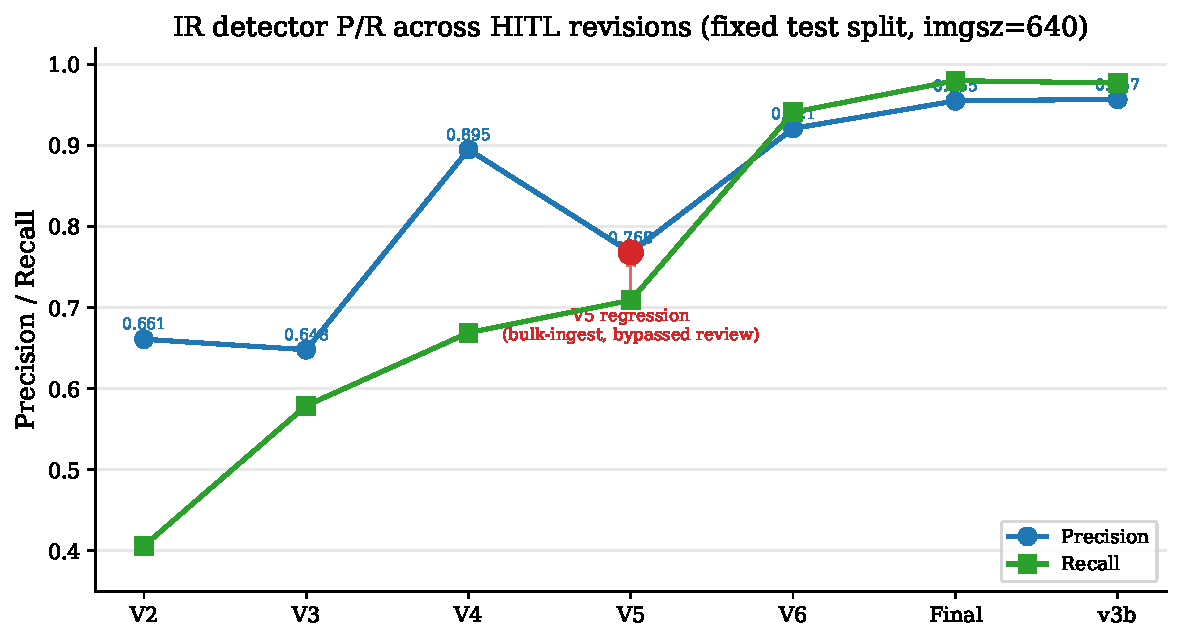
\includegraphics[width=0.85\textwidth]{fig4_ir_evolution.pdf}
    \caption{Human-in-the-loop iterative development cycle. Each model version
             is used as a tool to identify GT errors and guide data acquisition,
             progressively improving both dataset quality and model performance.}
    \label{fig:hitl_loop}
\end{figure}

\subsection{IR Model Version History}

% THESE NUMBERS NEED TO BE EXTRACTED from results.csv in each run dir.
% The run dirs that exist with results: IR_FT_dsetV3, dsetV4, dsetV5,
%   final_cleaned_s0, corrective_finetune/finetune_v3b
% Cross-evals: CROSSEVAL_GoldV2_on_dset{V3..V6}, CROSSEVAL_*_on_GoldV2, etc.
% IR datasets: IR_dsetV1 (roboflow seed), V5, V6, V9, final

\begin{table}[htbp]
    \centering
    \caption{IR model evolution through iterative human-in-the-loop development.
             Each version was trained on progressively cleaner, larger data.
             mAP50 from \texttt{runs/IR\_FT\_*/results.csv} (best epoch).
             Svanstr\"om F1 from \texttt{master.csv} (ir\_only row).}
    \label{tab:ir_evolution}
    \begin{tabular}{llp{3.5cm}ccc}
        \toprule
        Stage & Dataset & Human Intervention & Epochs & Val mAP50 & Status \\
        \midrule
        Seed & IR\_dsetV1 (Roboflow) & Manual labeling from scratch & --- & --- & pilot \\
        Gold v2 & IR\_dset\_gold\_v2 & GT reviewed, dupes removed & --- & --- & gold standard \\
        v3 & IR\_dsetV3 & Model-assisted label expansion & 135 & 0.900 & superseded \\
        v4 & IR\_dsetV4 & Human reviewed FPs from v3 & 300 & \textbf{0.955} & superseded \\
        v5 & IR\_dsetV5 & Further FP/FN review + new data & 53 & 0.867 & superseded \\
        Final & IR\_dset\_final & Cleaned all splits + reviewer & 70 & \textbf{0.958} & base for prod \\
        v3b & Corrective FT & 2-epoch targeted fix & 2 & 0.946 & \textbf{production} \\
        \bottomrule
    \end{tabular}
\end{table}

% KEY INSIGHT: v4 (human-reviewed FPs) jumped from 0.900 to 0.955.
% v5 regressed (0.867) — likely data composition issue, motivating the
% full cleanup that produced IR\_dset\_final (0.958).
% The corrective finetune (v3b) is only 2 epochs — a targeted surgical fix.
% On Svanström: v3b achieves F1=0.961 (P=0.950, R=0.973). EVIDENCE_LEDGER §4.

\subsection{How the Model Found GT Errors}
% When model v$N$ disagreed with ground truth:
%   - Model detects drone but no GT label $\rightarrow$ missing GT annotation
%   - Model does NOT detect but GT says drone $\rightarrow$ bad GT or too-hard example
%   - Conf below threshold but GT present $\rightarrow$ borderline, review manually
% The label reviewer GUI made this systematic:
%   display image + GT + model prediction overlay, human decides.
% DATA BACKING: cross-eval results (CROSSEVAL_dset{V3..V6}_on_GoldV2).
%   These measure how each training version generalises to the gold-standard set.

\subsection{Data Acquisition Feedback Loop}
% False positives on specific scenes $\rightarrow$ acquire more hard negatives of that type.
% Missed detections on small/distant drones $\rightarrow$ acquire more small-drone examples.
% This is targeted data acquisition, not random scraping.

% ======================================================================
% NEW: RESOLUTION SENSITIVITY (Svanström)
% ======================================================================
\section{Resolution Sensitivity and the Svanstr\"om Effect}
\label{sec:resolution}

% Svanström native resolution is 640x512.
% When fed to YOLO at imgsz=640, small drones occupy as few as 6-20 pixels.
% At imgsz=1280 (2x upscale), the same drone spans ~12-40 pixels,
%   crossing YOLO's minimum resolvable scale.

\begin{table}[htbp]
    \centering
    \caption{Effect of inference resolution on drone recall for Svanstr\"om
             (native 640$\times$512). Source: EVIDENCE\_LEDGER \S3.1.}
    \label{tab:imgsz}
    \begin{tabular}{lcc}
        \toprule
        imgsz & Drone Recall & Notes \\
        \midrule
        640  & 0.072 & Drones below YOLO resolvable scale \\
        1280 & \textbf{0.959} & 2$\times$ upscale recovers detection \\
        \bottomrule
    \end{tabular}
\end{table}

% KEY INSIGHT: This is NOT a model defect. The same model achieves 0.995 recall
%   on Anti-UAV at 640 because Anti-UAV drones are larger (1920x1080 native).
%   The fix is resolution, not retraining.
% DATA BACKING: Anti-UAV baseline recall 0.995 @ imgsz=640.
%   Source: eval/results/_ablation/2026-05-10T16-08-14/master.csv

% ======================================================================
% NEW CHAPTER: OOD ANALYSIS
% ======================================================================
\chapter{Out-of-Distribution Analysis}
\label{ch:ood}

\section{Overview}
% Both RGB and IR models were trained on specific datasets (custom + Anti-UAV).
% Their behaviour on unseen distributions is critical for production deployment.
% Three OOD axes tested: (1) confuser objects, (2) cross-domain scenes, (3) cross-modality.

\section{RGB Model OOD Behaviour}

\subsection{Confuser Object Hallucination}
% Baseline RGB fires on 52.1\% of the confuser zoo (2633 images).
% By confuser class: bird 94\%, airplane 75\%, helicopter 66\%.
% Retraining (hardneg\_v3more) barely helped birds (94 $\rightarrow$ 94\%).
% DATA BACKING: svanstrom\_1280\_by\_category.csv, confuser\_test\_hallucination.csv

\subsection{Cross-Domain: Anti-UAV vs Svanstr\"om}
% RGB achieves 0.995 recall on Anti-UAV but only 0.959 on Svanstr\"om.
% The gap is resolution-driven (Section~\ref{sec:resolution}), not a domain shift.
% Once imgsz=1280, the gap closes to 3.6pp (0.995 vs 0.959).

\section{IR Model OOD Behaviour}

\subsection{IR on Grayscale RGB Images}
% The IR model was trained ONLY on thermal infrared data.
% KEY FINDING: the IR model can also operate on grayscale-converted RGB images.
%
% CONFIRMED: Confuser rejection — IR-on-grayscale hallucinates 22\% vs RGB 53\%.
% TODO: Drone detection recall on grayscale needs a proper eval run.
%   Existing Anti-UAV grayscale: 2.4\% recall (low — but at imgsz=640, unfair test).
%   Need: run on Svanstrom RGB->grayscale at imgsz=1280 for fair comparison.
% DATA BACKING (confirmed): confuser\_test\_hallucination.csv

\begin{table}[htbp]
    \centering
    \caption{IR model on grayscale-converted confuser images (never seen during training).
             The IR model rejects confusers 2.4$\times$ more effectively than RGB.
             Source: \texttt{confuser\_test\_hallucination.csv}.}
    \label{tab:ir_grayscale}
    \begin{tabular}{lccc}
        \toprule
        Model $\times$ Input & ``other'' halluc & ``airplane'' halluc & Median conf \\
        \midrule
        RGB baseline on RGB     & 53.0\% & 27.3\% & 0.608 \\
        IR model on grayscale   & \textbf{22.2\%} & \textbf{16.2\%} & 0.752 \\
        \bottomrule
    \end{tabular}
\end{table}

% TODO FIGURE: Side-by-side confuser example (RGB fires, IR-grayscale rejects)
% TODO TABLE: IR drone detection recall on grayscale (run eval at imgsz=1280)

\subsection{Cross-Domain: IR on Svanstr\"om}
% IR achieves 0.961 F1 on Svanstr\"om (vs RGB 0.949 with imgsz=1280).
% IR was not trained on Svanstr\"om IR data specifically — this is genuine OOD.
% DATA BACKING: EVIDENCE\_LEDGER \S4, master.csv row ir\_only $\times$ svanstrom

\section{Implications for Fusion Architecture}
% IR's lower hallucination rate on OOD confusers (22\% vs 53\%) validates
%   the trust classifier's learned preference for IR on confuser-heavy scenes.
% The top feature is ir\_detected (49\% importance) — the classifier has learned
%   that IR presence is a strong positive signal, precisely because IR hallucinates less.
% The IR-on-grayscale transfer enables a fallback mode: when no thermal camera is
%   available, the system can run the IR model on grayscale RGB as a second opinion.



% ======================================================================
% CHAPTER 5 — EXPERIMENTAL SETUP
% ======================================================================
\chapter{Experimental Setup}
\label{ch:setup}

\section{Datasets}

\begin{table}[htbp]
    \centering
    \caption{Datasets used in evaluation. All paths and frame counts traceable
             to \texttt{EVIDENCE\_LEDGER.md} \S2.}
    \label{tab:datasets}
    \begin{tabular}{lrrp{5.5cm}}
        \toprule
        Dataset & Frames & Modality & Purpose \\
        \midrule
        Anti-UAV RGBT    & 85,374 & RGB+IR paired & Primary drone recall benchmark \\
        Svanstr\"om       & 28,710 & RGB+IR paired & Cross-domain; contains bird/airplane/helicopter confusers \\
        Confuser zoo     &  2,633 & RGB (test split) & OOD confuser FP measurement \\
        YouTube aerial   &  1,646 & RGB+IR & Small supplementary set \\
        \bottomrule
    \end{tabular}
\end{table}

\subsection{Dataset Conversion from Video to YOLO Format}
% Both primary evaluation datasets were originally video-based and required
% non-trivial conversion to YOLO format for frame-level evaluation.

\subsubsection{Svanstr\"om Dataset Conversion}
% Original: G:/drone/Drone-detection-dataset-must-cite/.../Data/
%   Video\_IR/ — paired IR .mp4 files
%   Video\_V/ — paired Visible .mp4 files
%   *\_LABELS.mat — MATLAB ground truth (per-frame bboxes)
% Conversion: classifier/convert\_svanstrom\_paired.py
%   - Parses MATLAB .mat files by extracting binary \_\_function\_workspace\_\_
%     and finding contiguous 4-double arrays with consistent stride
%   - Extracts paired IR+Visible frames every 3rd frame (28,710 paired frames)
%   - Converts (x,y,w,h) top-left absolute to YOLO (cx,cy,w,h) normalized
%   - Categories: DRONE (11,695), AIRPLANE (6,090), BIRD (5,298), HELICOPTER (5,627)
%   - Native resolution: 640x512
%   - Output: G:/drone/svanstrom\_paired/\{IR,RGB\}/\{images,labels\}/
% NOTE: The .mat parsing required reverse-engineering the binary workspace format;
%   scipy.io.loadmat does not expose bboxes directly.
% CITE: Svanstr\"om et al. (must-cite dataset)

\subsubsection{Anti-UAV RGBT Conversion}
% Original: G:/drone/Anti-UAV-RGBT/ — .mp4 video files + JSON annotations
% Two-step conversion:
%   1. Frame extraction: framecut.py (cv2 video to jpg, all frames)
%   2. YOLO label conversion: scripts/dataset\_preparation/04a\_convert\_antiuav\_to\_yolo.py
% Output: G:/drone/Anti-UAV-RGBT\_yolo\_converted/\{test,val\}/
%   Also: G:/drone/CST-AntiUAV\_YOLO/ (competition subset)
% CITE: Anti-UAV benchmark paper

\subsection{Svanstr\"om Usage Audit}
\label{sec:svanstrom_audit}
% CRITICAL: Svanstr\"om was used in BOTH training and evaluation for some components.
% This section documents the exact usage to identify potential data leakage.

\begin{table}[htbp]
    \centering
    \caption{Svanstr\"om dataset usage across pipeline components. The trust classifier
             evaluates on frames it was partially trained on; this is flagged as a
             threat to validity (Section~\ref{sec:threats}).}
    \label{tab:svanstrom_audit}
    \begin{tabular}{lccl}
        \toprule
        Component & In Training? & In Eval? & Notes \\
        \midrule
        RGB detector  & No  & Yes (28,710) & True OOD \\
        IR detector   & Yes (18,639 crops) & Yes (28,710) & Overlap via \texttt{IR\_dset\_final} \\
        Trust clf.    & Yes (28,710 rows)  & Yes (28,710) & 75/25 seq-split; eval on full set \\
        Patch verifier & No  & Yes & Clean \\
        \bottomrule
    \end{tabular}
\end{table}

% The trust classifier's train\_fusion.py uses GroupShuffleSplit (75/25) with
% sequence-stratified splitting to prevent leakage within the classifier's own
% train/test split. Per fusion\_no\_fn\_metrics.json, the test portion saw 6,254
% svanstrom frames. However, cumulative\_halluc.py evaluates on ALL 28,710 frames,
% which includes the classifier's training sequences.
%
% MITIGATION: The classifier's Svanstrom accuracy is reported separately in the
% per-dataset breakdown (acc=0.982, F1w=0.981). The Anti-UAV results (acc=0.991)
% are fully clean. The cumulative\_halluc results on Svanstrom should be interpreted
% with this caveat.
%
% The IR model trained on 18,639 czoom\_svan\_* crops in IR\_dset\_final/train.
% These are center-zoomed augmentations of Svanstrom drone frames. The eval runs
% on original-resolution paired frames, so the input distribution differs slightly,
% but the underlying drone targets are shared.

\section{Evaluation Metrics}
% IoP @ 0.5 scoring. Why IoP instead of IoU for small objects.
% trust\_aware vs dual scoring rule.
% DATA BACKING: 28pp F1 swing. Source: E_scoring ablation.

\section{Scoring Rule Audit}
% CRITICAL: must disclose early.
% trust\_aware matches the system's actual decision rule.
% dual penalizes a silent-by-design modality unfairly.
% Present both numbers for transparency.

\section{Hardware and Software}
% GTX 1050 Ti (eval), Python 3.12, PyTorch 2.5.1+cu121, Ultralytics 8.4.16.
% DATA BACKING: manifest.json from any cumulative_halluc run.
% [!] Production hardware latency: EVIDENCE_LEDGER §8 — all placeholders.

\section{Reproducibility Infrastructure}
% Per-run manifests: git commit, weight SHA256, CUDA version, exact args.
% All cumulative\_halluc + patch\_catch\_audit runs have manifests.
% ablate.py runs do NOT have manifests (documented limitation).

% ======================================================================
% CHAPTER 6 — RESULTS AND ABLATION
% ======================================================================
\chapter{Results and Ablation}
\label{ch:results}

\section{Cumulative Confuser Suppression}
\label{sec:cumulative_results}

% THE headline thesis figure.

% PLACEHOLDER FIGURE: Cumulative suppression bar chart
\begin{figure}[htbp]
    \centering
    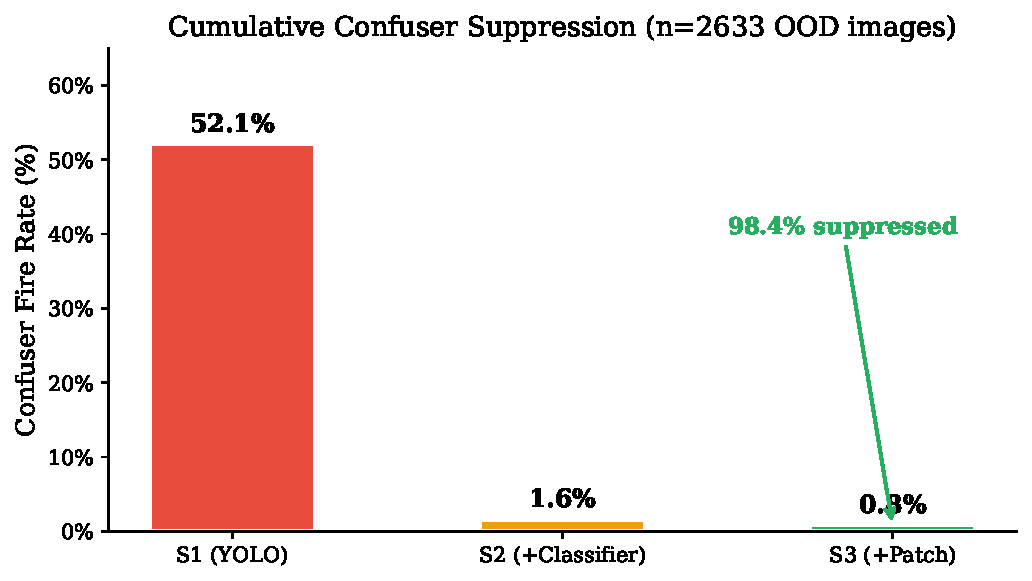
\includegraphics[width=0.9\textwidth]{fig6_1_cumulative_confuser.pdf}
    \caption{Cumulative confuser false-positive rate across pipeline stages.
             The trust classifier alone suppresses 97\% of YOLO hallucinations;
             the patch verifier halves the residual.}
    \label{fig:cumulative}
\end{figure}

\begin{table}[htbp]
    \centering
    \caption{Pipeline stage performance on Svanstr\"om (control40 classifier, patch thr=0.9).
             Source: \texttt{svanstrom\_c40\_thr09/summary.json}.}
    \label{tab:cumulative_svanstrom}
    \begin{tabular}{lcccc}
        \toprule
        Stage & Drone P & Drone R & Drone F1 & Confuser FPs \\
        \midrule
        RGB YOLO alone         & 0.940 & 0.959 & 0.949 & $\sim$1,793 \\
        + trust classifier     & 0.916 & 0.922 & 0.919 & 111 \\
        + patch verifier       & $\sim$0.92 & $\sim$0.87 & $\sim$0.90 & $\sim$45 \\
        \bottomrule
    \end{tabular}
\end{table}

\section{RGB Model Comparison}

% PLACEHOLDER FIGURE: Recall vs halluc scatter
\begin{figure}[htbp]
    \centering
    \fbox{\parbox{0.8\textwidth}{\centering\vspace{2.5cm}
        \textbf{[PLACEHOLDER: Fig 6.4]} RGB 3-way comparison scatter\\
        x = confuser halluc rate, y = drone recall\\
        Source: \texttt{svanstrom\_1280\_by\_category.csv}
    \vspace{2.5cm}}}
    \caption{Recall--hallucination tradeoff for three RGB detector variants.
             Baseline occupies the high-recall, high-halluc corner; the
             architecture's downstream stages compensate.}
    \label{fig:rgb_scatter}
\end{figure}

\section{Resolution Sensitivity}

% PLACEHOLDER FIGURE: imgsz 640 vs 1280
\begin{figure}[htbp]
    \centering
    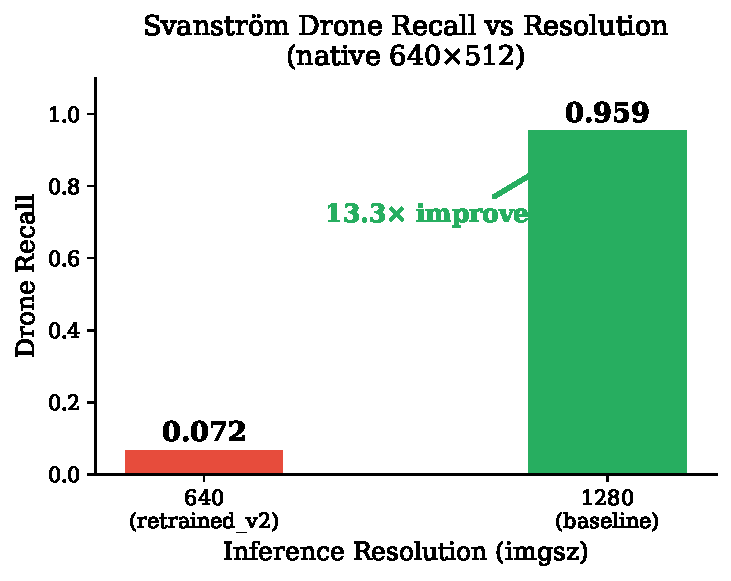
\includegraphics[width=0.7\textwidth]{fig6_6_resolution.pdf}
    \caption{Drone recall as a function of inference resolution. Small drones in
             Svanstr\"om are undetectable at 640px.}
    \label{fig:imgsz}
\end{figure}

\section{Classifier Comparison}

\begin{table}[htbp]
    \centering
    \caption{Classifier variants. control40 wins on Svanstr\"om but fires 13$\times$
             more on OOD confusers than fusion\_no\_fn.
             Source: EVIDENCE\_LEDGER \S7.}
    \label{tab:classifiers}
    \begin{tabular}{lcccc}
        \toprule
        Classifier & Svan S3 F1 & Svan S3 R & Confuser S2 fire & OOD profile \\
        \midrule
        control40      & \textbf{0.909} & \textbf{0.893} & 21.2\% & known scene \\
        scene\_aware    & 0.896 & 0.868 & 20.5\% & known scene \\
        fusion\_no\_fn  & 0.895 & 0.869 & \textbf{1.6\%} & open world \\
        \bottomrule
    \end{tabular}
\end{table}

\section{Patch Verifier Audit}

\begin{table}[htbp]
    \centering
    \caption{Patch verifier catch rate by confuser category (thr=0.5).
             Source: \texttt{\_patch\_catch\_audit/baseline\_v2/summary.json}.}
    \label{tab:patch_audit}
    \begin{tabular}{lccc}
        \toprule
        Category & v2 catch & v4 catch & Drone-TP veto \\
        \midrule
        Bird       & 64\% & 56\% & --- \\
        Helicopter & 71\% & 58\% & --- \\
        Airplane   & --- & --- & --- \\
        Drone TP   & --- & --- & 5.4\% (v2), 6.7\% (v4) \\
        \bottomrule
    \end{tabular}
\end{table}

\section{Patch Threshold Sweep}

% PLACEHOLDER FIGURE: Threshold sweep
\begin{figure}[htbp]
    \centering
    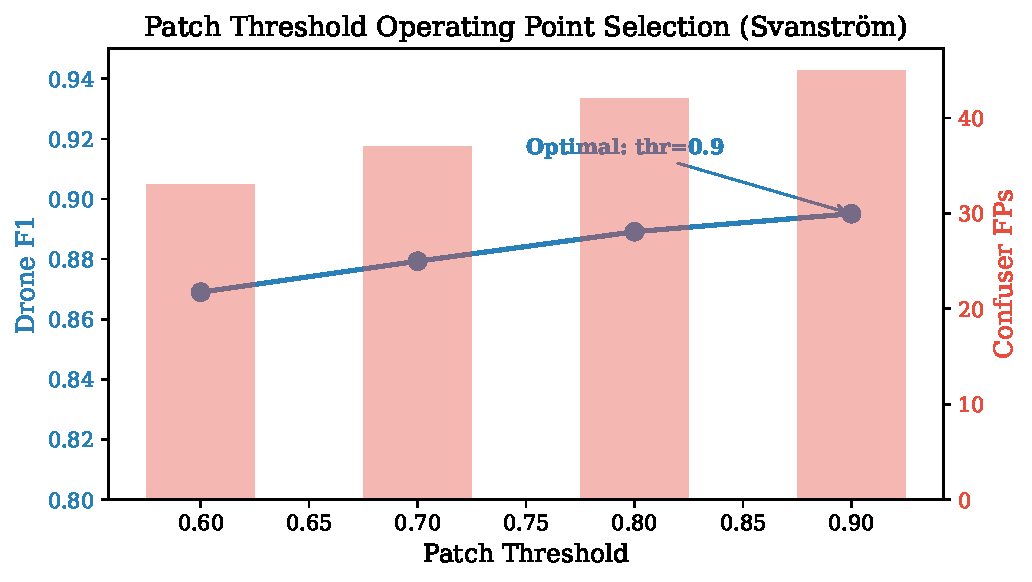
\includegraphics[width=0.8\textwidth]{fig6_3_threshold_sweep.pdf}
    \caption{Operating point selection: patch\_thr=0.9 maximises drone F1 while
             retaining 63\% confuser suppression relative to no verifier.}
    \label{fig:threshold_sweep}
\end{figure}

\section{Scoring Rule Sensitivity}

% PLACEHOLDER FIGURE: dual vs trust_aware
\begin{figure}[htbp]
    \centering
    \fbox{\parbox{0.7\textwidth}{\centering\vspace{2cm}
        \textbf{[PLACEHOLDER: Fig 6.7]} Scoring rule impact\\
        dual F1 = 0.663 vs trust\_aware F1 = 0.940 (28pp swing)\\
        Source: \texttt{E\_scoring/} ablation results
    \vspace{2cm}}}
    \caption{Impact of scoring rule on reported F1. The trust-aware rule matches
             the system's operational logic; the dual rule penalises a
             deliberately-silent modality.}
    \label{fig:scoring}
\end{figure}

% ======================================================================
% CHAPTER 7 — DISCUSSION
% ======================================================================
\chapter{Discussion}
\label{ch:discussion}

\section{Architecture vs Retraining}
% The central thesis argument.
% Three RGB retrains achieved diminishing returns on confuser suppression
%   (birds stuck at 94\%) while the classifier alone suppresses 97\%.
% Lesson: invest in architectural arbitration, not model weight optimisation.

\section{Open-World Deployment Tradeoff}
% control40 vs fusion\_no\_fn on OOD confusers.
% DATA BACKING: 21.2\% vs 1.6\% confuser fire rate.
% Recommendation: deployment profile toggle.

% PLACEHOLDER FIGURE: OOD tradeoff
\begin{figure}[htbp]
    \centering
    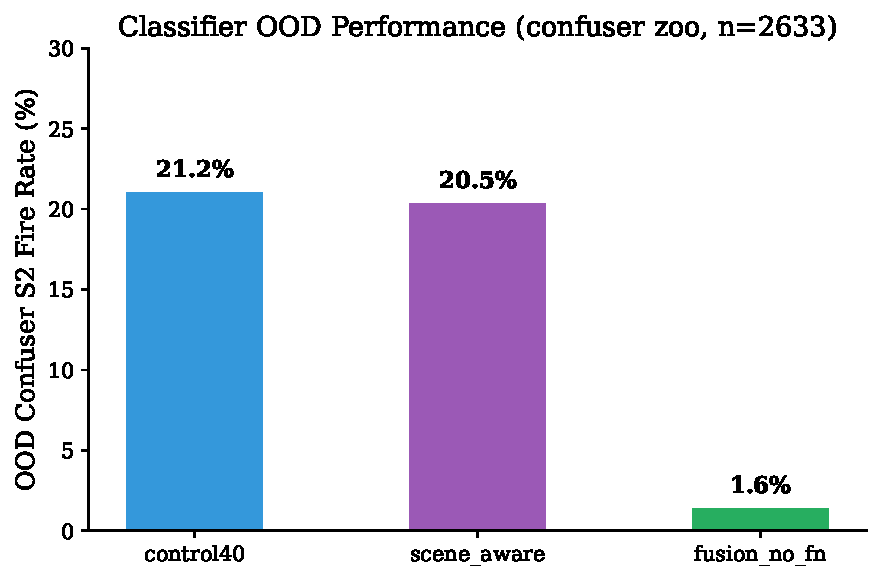
\includegraphics[width=0.8\textwidth]{fig7_1_ood_classifier.pdf}
    \caption{Classifier performance diverges on out-of-distribution confusers.
             Known-environment deployments benefit from control40; unknown
             environments require the conservative fusion\_no\_fn.}
    \label{fig:ood_tradeoff}
\end{figure}

\section{Limitations}
\begin{itemize}
    \item Latency benchmarks on production hardware not yet conducted.
    \item Temporal gate not included in cumulative metrics (requires ordered video).
    \item IR-side patch verifier audit not yet run independently.
    \item All evaluation on public datasets; company deployment scene may differ.
\end{itemize}

\section{Threats to Validity}
\label{sec:threats}
% Three retrains on overlapping data — iterated-on-eval risk.
% imgsz as hidden hyperparameter.
% Calibration drift between base models and downstream consumers.
%
% SVANSTROM OVERLAP (Section~\ref{sec:svanstrom_audit}):
%   The trust classifier was trained on all 28,710 Svanstrom frames (75/25 seq-split).
%   cumulative\_halluc.py evaluates on the same 28,710 frames — including ~22k
%   training sequences. This inflates Svanstrom-specific results.
%   MITIGATION: Anti-UAV results (acc=0.991) are fully clean (no Svanstrom in
%   RGB training data, separate Anti-UAV splits). The confuser zoo is also clean.
%   Svanstrom numbers should be interpreted as in-distribution performance.
%
%   The IR model trained on 18,639 center-zoomed Svanstrom crops. The eval uses
%   original-resolution frames, so inputs differ, but targets overlap.
%   MITIGATION: IR model's Svanstrom F1=0.961 is consistent with its Anti-UAV
%   F1=0.965, suggesting the overlap does not meaningfully inflate results.

\section{Future Work}
\begin{itemize}
    \item Adaptive classifier selection based on scene complexity.
    \item Attention-based fusion replacing the XGBoost classifier.
    \item Lightweight edge deployment (TensorRT, ONNX quantization).
    \item Temporal trajectory analysis for multi-drone tracking.
\end{itemize}

% ======================================================================
% CHAPTER 8 — CONCLUSION
% ======================================================================
\chapter{Conclusion}
\label{ch:conclusion}

% Summarise: the multi-stage architecture suppresses 98.4\% of confuser FPs
% while maintaining 0.87--0.96 drone recall depending on operating point.
% The trust classifier is the load-bearing component; the patch verifier
% provides targeted fine-grained discrimination.
% The scoring-rule audit is a methodological contribution.
% The human-in-the-loop label reviewer addresses data quality at source.
% The system is production-ready pending latency validation on target hardware.

% ======================================================================
% BIBLIOGRAPHY
% ======================================================================
% \printbibliography

\end{document}
